\documentclass[12pt]{article}

\usepackage{amsmath, graphicx}
\usepackage[margin=1in]{geometry}
\usepackage[font=footnotesize]{caption}

\begin{document}
\nocite{*}

\title{Progress Report - Super Mario Bros with Deep Reinforcement Learning}

\author{
  Matthew Chen
  \and
  Isabel Bush
}
\date{}
\maketitle


\section{Abstract}

For this project we are implementing various reinforcement learning algorithms to create learning agents to effectively play a variant of the classic Super Mario Bros game. The game is challenging from an AI standpoint as the environment is stochastic with randomly generated levels, and the state space is large. To address these challenges we will use Q-learning with various Q-function approximations ranging from simplistic feature extractors to deep learning implementations.


\section{Models}

\begin{figure}
\centering
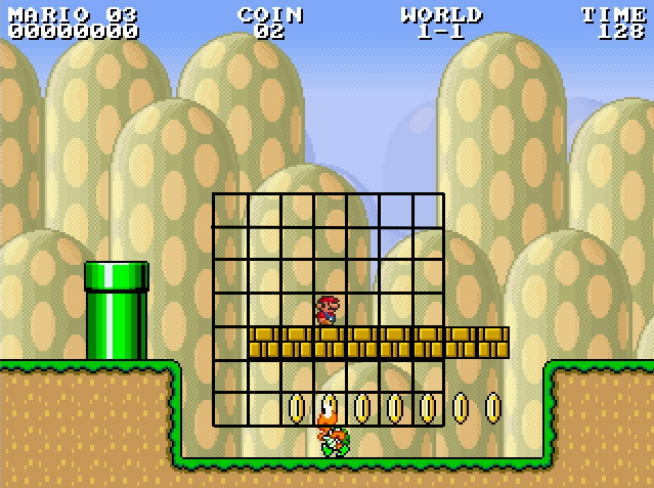
\includegraphics[scale=0.5]{imgs/mario_grid}
\caption{A component of the game state is a small grid centered around Mario indicating objects nearby. In the actual simulation, the grid is 22 x 22 cells, where each cell is the size of a single block \cite{karakovskiy}.}
\label{mario_grid}
\end{figure}

We are running several variants of the Q learning algorithm with differing function approximations. All variants use an epsilon-greedy policy to choose an action at each state.

Our state is defined as a vector of all observed attributes of the game. This can be divided into two components. In the first component are meta data features which include distance to the finish, time left, and Mario state. These features describe the progression of the game. The second component is a 22 x 22 grid which is provided by the simulator at each time step, as shown in Figure \ref{mario_grid}. The grid can be thought of as a low detail/resolution view of the game. The entire grid is centered around Mario and each cell corresponds to objects in that relative position to Mario (blocks, mushrooms, monsters, gap, etc).

Actions correspond to combinations of the original buttons which could be pressed for the player to interact with the game. The game uses a set of six buttons which can be toggled on and off during a given time-step to make Mario move forward, jump, throw a fireball, etc. Since combinations of buttons are possible, we have defined our set of possible actions as all binary combinations of the six buttons leading to $2^6 = 64$ distinct actions.

The reward at each time-step is calculated as the change in fitness score over that time-step due to the action taken at the previous state. The fitness score takes into account distance passed and coins collected.

\subsection{Identity Function}

Our first learning agent maps the full state representation vector to the best action to take from that state. Since the state space is very large (the state vector has length $733$, which yields upwards of $2^{733}$ distinct states) and many states are unlikely to be seen (creating a sparse feature vector), we stored the state-action mapping in a hashmap to allow for quick access and efficient space usage.

While this is a simple model, it has a few shortcomings. First, since this simple Q learning model maps directly from states to actions, no generalization may be made to unseen states. The best action to take from each state must be learned independently, and the agent will choose a random action for any new state (even if very similar to a past state). This makes learning slow and inefficient. Second, an implementation shortcoming of this model is that the large feature vector consisting of all possible states can overflow memory. This limits the number of learning trials that may be run as the memory-usage grows with each new state.

\subsection{Linear Approximation}

To overcome the shortcomings of the identity function model, we implemented a linear approximation model. Rather than map directly from states to actions, this model defines a feature vector over the states and actions and calculates the optimal Q value at each time-step as the dot product of the current state/action feature vector and learned weights. 

The feature vector consists of indicator values for each element of the state vector and every possible action. This yields a feature vector of length $stateVectorLength * possibleActions = 733 * 64 = 46,912$. While still large, this is much less than the identity feature vector and can easily fit in memory. And more importantly, this allows the agent to generalize to unseen states and learn more quickly.

\subsection{Neural Network}

We will try two neural network representations for approximating the Q function. In this representation we will use several fully-connected layers, with either logistic units or rectifier units. This network will take as input the state vector described above and output a Q score approximation.

Additionally, we will use playback memory as defined in \cite{mnih}. We will store the previous N observations from the game. We then sample from these observations during a single update to perform mini-batch gradient descent. This method should help mitigate the problem of correlated features from time windows and aid in the convergence of the weights.

\section{Initial Results}

\begin{figure}
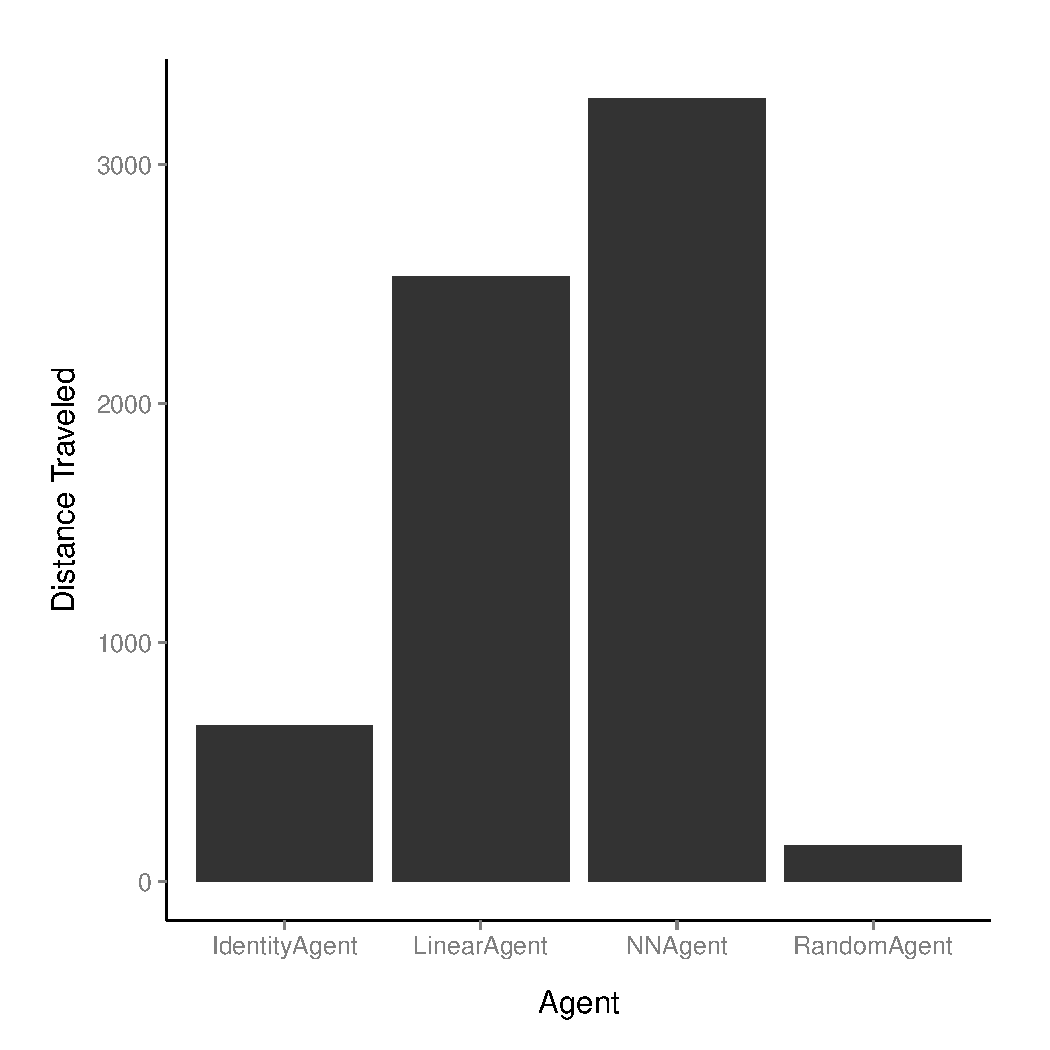
\includegraphics[scale=0.5]{imgs/dist_bar.pdf}
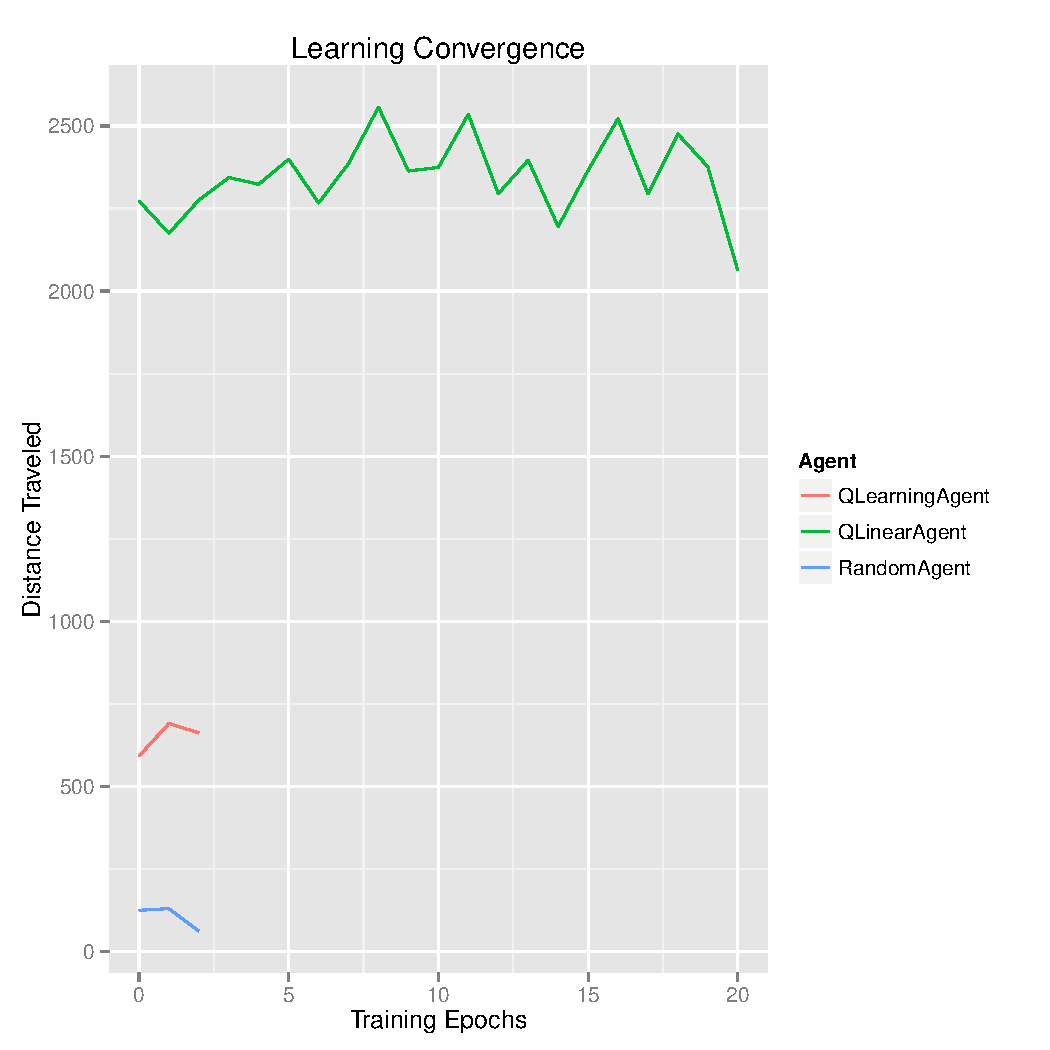
\includegraphics[scale=0.5]{imgs/dist_line.pdf}
\caption{Learning statistics showing comparison between different agents by mean progress before end of game}
\label{agent_comp}
\end{figure}

We implemented initial versions of the Identity and Linear Approximation Agents, as well as a baseline random agent that chooses a random action at each step. Preliminary results show that both models are able to learn some of the game's goals and outperform the random agent by a large margin as shown in Figure \ref{agent_comp}.

The Identity Agent was able to run for about 200 trials before running out of memory (where each trial is a full game and consists of about 1000 time-steps). At the start of learning, Mario jumps around aimlessly performing random actions. By the end of the 200 trials, the agent has learned to move forward from some states and thus makes progress. However, since there is no generalization, the agent still performs random actions from some states and the game usually ends due to time-out. 

The distance travelled over the trials for the agents can be seen in the Learning Convergence graph in Figure \ref{agent_comp}. While there is much variability, the trend is positive for the Identity Agent. Over the last 50 trials, the Identity Agent travelled an average distance of 710 with an average fitness score of 1,561. This is significantly better than the baseline random agent, which travels an average distance of 127 with an average fitness score of 257.

Due to generalization of state features, the Linear Agent learns much faster than the Identity Agent, as can be seen by the higher distance travelled even during the first few training epochs. The rate is faster despite a much lower learning rate (step-size), which was needed to keep the weights from diverging. The Linear Agent is able to progress farther on average than the Identity Agent (generalizing the desire to move forward to many different states) and thus usually completes the level or dies from a monster rather than hitting the timeout. The Linear Agent travels an average distance of 2,360 with an average fitness score of 5,140, far outperforming both the random agent and Identity Agent.

\section{Future Work}

The following are next steps in our project:

\begin{enumerate}
\item Implement Neural Network Agent
\item Record training statistics for all agents
\item Compare performance and run times of all agents
\item Benchmark our results against competition results
\end{enumerate}

\begin{thebibliography}{1}

\bibitem{karakovskiy} S. Karakovskiy, J. Togelius {\em The Mario AI Benchmark and Competitions} 2012.

\bibitem{mnih} V. Mnih, K. Kavukcuoglu, D. Silver, A. Graves, I. Antonoglou, D. Wierstra, M. Riedmiller {\em Playing Atari with Deep Reinforcement Learning} 2013.

\end{thebibliography}

\end{document}